\documentclass[conference]{IEEEtran}
%\documentclass[dvipdfmx,conference]{IEEEtran}
\IEEEoverridecommandlockouts
% The preceding line is only needed to identify funding in the first footnote. If that is unneeded, please comment it out.
\usepackage{cite}
\usepackage{amsmath,amssymb,amsfonts,amsthm}
\usepackage{algorithmic}
\usepackage{graphicx}
\usepackage{textcomp}
\usepackage{xcolor}
\usepackage{bbm}
\usepackage{dsfont}
\usepackage{bm}
\usepackage{algorithm}
\usepackage{algorithmic}

\usepackage{color}

\newtheorem{thm}{Theorem}
\newtheorem{lem}[thm]{Lemma}
\newtheorem{prop}[thm]{Proposition}
\newtheorem{cor}[thm]{Corollary}
\newtheorem{conj}[thm]{Conjecture}
\newtheorem{definition}[thm]{Definition}
\newtheorem{assumption}[thm]{Assumption}

\newcommand{\R}{\mathbb{R}}
\newcommand{\one}{\mathds{1}}
\newcommand{\mat}[1]{\mathbf{#1}}
%\renewcommand{\vec}[1]{\mathbf{#1}}
\renewcommand{\vec}[1]{\bm{#1}}
\newcommand{\prox}{\operatorname{prox}}
\newcommand{\proj}{\operatorname{Proj}}
\newcommand{\argmin}{\operatorname{argmin}}
\newcommand{\changeHK}[1]{\textcolor{black}{#1}}

\newcommand{\changeSX}[1]{\textcolor{black}{#1}}

\def\BibTeX{{\rm B\kern-.05em{\sc i\kern-.025em b}\kern-.08em
T\kern-.1667em\lower.7ex\hbox{E}\kern-.125emX}}
\begin{document}

\title{Accelerated Majorization-Maximization algorithm with Dynamic Penalty Updating for Unbalanced Optimal Transport}

\author{\IEEEauthorblockN{Xun Su}
\IEEEauthorblockA{\textit{Graduate School of Fundamental Science and Engineering } \\
\textit{WASEDA University}\\
Tokyo, Japan \\
suxun$\_$opt@asagi.waseda.jp}
\and
\IEEEauthorblockN{Hiroyuki Kasai}
\IEEEauthorblockA{\textit{School of Fundamental Science and Engineering} \\
\textit{WASEDA University}\\
Tokyo, Japan \\
hiroyuki.kasai@waseda.jp}

}

\maketitle

\begin{abstract}
With the increasing applications of Optimal Transport (OT) in the machine learning field, the unbalanced optimal transport (UOT) problem, as a variant of optimal transport, has gained attention for its improved generality. There is an urgent need for fast algorithms that can efficiently handle large penalty parameters. In this paper, we prove that the recently proposed Majorize-Minimization algorithm for the UOT problem can be viewed as a form of the Bregman Proximal Descent, and we propose to use dynamic penalty updating to make the algorithm converge quickly even for large penalties. By using a dynamic scheme, we can successfully compute better and sparser solutions for the large penalty parameter and approach the computational speed of the well-known Sinkhorn's algorithm, which sacrifices accuracy by adding an entropy item.
\end{abstract}

\begin{IEEEkeywords}
Optimization, Optimal Transport, Unbalanced Optimal Transport, Majorization-Maximization Algorithm, Mirror Descent, Bregman Proximal Descent.
\end{IEEEkeywords}

\section{Introduction}
\label{sec:int}

Optimal transport (OT) has gained significant attention in the fields of machine learning and statistical learning due to its capacity to measure the distance between two probability measures. Combined OT methods have demonstrated superiority over traditional methods in areas such as domain adaptation \cite{Courty_PAMI_2017} and generative models \cite{arjovsky2017wasserstein}. Recently, OT theory has been applied to diverse technical fields, including graph analysis \cite{Huang_SigPro_2020,Huang_ICASSP_2021,Fang_AAAI_2023} and sequential data analysis \cite{Horie_EUSIPCO_2022}. The popularity of OT can be attributed to the introduction of Sinkhorn's algorithm \cite{Cuturi_NIPS_2013} for the entropy-regularized Kantorovich formulation problem, which has reduced the computational complexity associated with large-scale problems. However, the standard OT problem is limited to handling only {\it balanced} samples. To accommodate a wider range of applications with {\it unbalanced} samples, relaxed OT has been proposed, including partial OT (POT) \cite{ferradans2013regularized}, semi-relaxed OT (SROT) \cite{fukunaga_icassp2022,fukunaga_srsinkhorn}, and unbalanced optimal transport (UOT) \cite{Caffarelli_AM_2010,chizat2017scaling}. The UOT has been proposed as a method to replace equality constraints with KL divergence as a penalty function. It is solvable by adding an entropic regularization term and utilizing Sinkhorn's algorithm. Although it is fast, scalable, and differentiable, it is prone to instability and results in larger errors in solutions compared to other regularizers.

Recently, Chapel et al. proposed a Majorization-Maximization (MM) algorithm to solve the UOT problem without adding an entropy term by exploiting the connection between UOT and non-negative matrix factorization \cite{Chapel_NeurIPS_2021}. Although their algorithm is GPU compatible and computationally efficient, it produces a solution that is blurrier than that of Sinkhorn's algorithm and is slower, especially for large penalty terms. In this paper, we propose to combine the MM algorithm with a dynamic penalty method to speed up the optimization process. The dynamic method was first introduced by \cite{pmlr-v115-xie20b} in the OT community and has been adapted in Augmented Lagrangian methods for many years for faster convergence. Our approach is simple and effective, and significantly improves the computational speed of the MM algorithm for larger penalty terms.
Our contributions are:
\begin{itemize}
\item This paper proves that the MM algorithm for UOT can be derived from the Bregman Proximal Descent (BPD) algorithm with the theoretical step size.
\item This paper proposes to combine the MM algorithm with the dynamic penalty method to deal with the deterioration condition for a large penalization parameter. We call our proposed method the Dynamic Penalized MM Algorithm (DPMM). This modification is simple but enables a faster convergence. In addition, the obtainable results are less blurry.
\item The numerical evaluations on unbalanced and balanced samples demonstrate the effectiveness of our proposed DPMM and its accelerated variant. More concretely, our method achieves faster convergence comparable to the Sinkhorn's algorithm for balanced samples and surpasses it for unbalanced samples in accuracy. DPMM and its Nesterov acceleration variant DPAMM can produce solutions that have the same quality as Sinkhorn's algorithm.
\end{itemize}

\section{Preliminaries}
\subsection{Notation}
We use $\| \cdot \|_2$ to represent the Euclidean norm. $\mathbb{R}^n$ denotes $n$-dimensional Euclidean space, and $\mathbb{R}^n_+$ denotes the set of vectors in which all elements are non-negative. $\mathbb{R}^{n \times m}_+$ stands for the set of $n \times m$ matrices in which all elements are non-negative. We use $\Delta$ to represent the Hessian operator. We present vectors Aas bold lower-case letters $\vec{a},\vec{b},\vec{c},\dots$ and matrices as bold-face upper-case letters $\mat{A},\mat{B},\mat{C},\dots$. The $i$-th element of $\vec{a}$ and the element at the $(i,j)$ position of $\mat{A}$ are stated respectively as $a_i$ and ${A}_{i,j}$, the $i$-th column of $\mat{A}$ is represented as $\vec{a}_i$. In addition, $\one_n \in \mathbb{R}^n$ is the $n$-dimensional vector in which all elements are one. Additionally, we suggest vectorization for $\mat{A} \in \mathbb{R}^{n \times m}$ as lowercase letters $\vec{a} \in \mathbb{R}^{nm}$ and $\vec{a}=\text{vec}(\mat{A})=[{A}_{1,1}, {A}_{1,2}, \cdots, {A}_{m,n-1}, {A}_{m,n}]^T$, i.e., the concatenated vector of the transposed row vectors of $\mat{A}$.
%For $\vec{x}$ and $\vec{y}$ of the same size, $\langle \vec{x},\vec{y} \rangle = \vec{x}^T\vec{y}$ is the Euclidean dot-product between vectors.
For two matrices of the same size $\mat{A}$ and $\mat{B}$, $\langle \mat{A},\mat{B}\rangle={\rm tr}(\mat{A}^T\mat{B})$ is the Frobenius dot-product.

\subsection{Optimal Transport and Unbalanced Optimal Transport}
The {\it balanced} OT problem is defined as
\begin{eqnarray}
\label{Eq:Standard_OT}
\operatorname{OT}(\vec{a},\vec{b}) &:=& \min_{ \mat{T} \in \R_{+}^{n \times m}} \langle \mat{C}, \mat{T} \rangle \\
\text{subject\ to}&& \mat{T} \one_n= \vec{a}, \mat{T}^{T}\one_m = \vec{b}. \notag
\end{eqnarray}
By relaxing the constraints using the Kullback-Leibler (KL) divergence, we can obtain the UOT problem:
\begin{align}
\label{eq:uot}
&\operatorname{UOT}(\vec{a},\vec{b}) := \notag\\
&\min_{\mat{T} \in \R_{+}^{n \times m}} \langle \mat{C}, \mat{T} \rangle+ \tau \mathrm{KL}(\mat{T} \one_n,\vec{a}) + \tau \mathrm{KL}(\mat{T}^{T} \one_n,\vec{b}),
\end{align}
where $\mathrm{KL}(\vec{x},\vec{y})$ stands for the KL divergence between $\vec{x} \in \mathbb{R}_+^n$ and $\vec{y} \in \mathbb{R}_+^n$, which is defined as $\sum_i {x}_i \log {({x}_i/{y}_i)} - \vec{x}_i + {y}_i$.


\subsection{MM Algorithm for UOT problem}
For this UOT problem, Chapel et al. consider it as a composite optimization problem \cite{Chapel_NeurIPS_2021} given by
\begin{align}
\label{eq:reg}
\min_{\vec t \in \mat{R}^{nm}} ~ \left\{ f(\vec t) := g(\vec t) + h(\vec t)\right\},
\end{align}
where $g(\vec t) = \vec c^{T}\vec t$ and $h(\vec t) = \tau D_{\phi}(\mat H \vec t, \vec y)$. Here, $\vec y = [\vec a^{T}, \vec b^{T}]^{T} \changeSX{\in \mathbb{R}^{n+m}}$, $\mat H = [\mat {M}^{T}, \mat {N}^{T}]^{T} \changeSX{\in \mathbb{R}^{(n+m) \times nm}}$, and $\mat {M} $ and $\mat {N}$ are the indicator matrices consist of 1 and 0 to computing the sum of $\vec t$ according to rows and columns in $\mat T$ form. Under this formulation, they propose an MM algorithm to solve the UOT problem, by building an auxiliary function $G_\tau(\boldsymbol{t}, \tilde{\boldsymbol{t}})$ for divergence $D_{\phi}$ on the assumption of $\tilde{Z}_{i, j}=H_{i, j} \tilde{t}_j/\sum_l H_{i, l} \tilde{t}_l$. This auxiliary function $G_\tau(\boldsymbol{t}, \tilde{\boldsymbol{t}})$ is defined as
\begin{eqnarray}
\label{eq:af}
G_\tau(\boldsymbol{t}, \tilde{\boldsymbol{t}})&=&\sum_{i, j} \tilde{Z}_{i, j} \phi\left({H_{i, j} t_j}/{\tilde{Z}_{i, j}}\right)\notag\\
&&+\sum_j\left[\frac{c_j}{\tau}-\sum_i H_{i, j} \phi^{\prime}\left(y_i\right)\right] t_j\notag\\
&&+\sum_i\left[\phi^{\prime}\left(y_i\right) y_i-\phi\left(y_i\right)].\right.
\end{eqnarray}

By minimizing $G_{\tau}( \vec t, \vec t^{k}) $, they obtain the following updating formula in a matrix form
\begin{align}
\label{eq:update}
&\mat{T}^{(k+1)}=\notag\\
&\operatorname{diag}\!\left(\frac{\vec a}{\mat{T}^{(k)} \one_m}\right)^{\frac{1}{2}}
\!\!\left(\!\mat{T}^{(k)} \!\odot\! \exp \left(-\frac{\mat C}{2 \tau}\right)\!\right)
\operatorname{diag}\!\left(\!\frac{\vec{b}}{\mat{T}^{(k) \top} \one_n}\!\right)^{\frac{1}{2}}\!\!\!.\notag\\
\end{align}

It is worth noting that the updating formula presented in (\ref{eq:update}) bears remarkable similarities with the widely popular Sinkhorn's algorithm, as it relies solely on matrix multiplication. While Sinkhorn's algorithm solves (\ref{eq:uot}) with an additional regularization term $\epsilon \mat H(\mat T) = \epsilon \langle \mat T,\ln(\mat T - 1)\rangle$ using an alternative matrix multiplication method, it shares a similar computational structure with MM algorithm. This feature also allows for the use of GPU acceleration to speed up the computation process.

\section{Proposed Algorithm}
\subsection{MM algorithm and Its BPD algorithm}
Traditional Gradient descent cannot be applied to some Banach Spaces in which the dual space is not consistent with the primal one. Mirror Descent \cite{doi:10.1137/1027074, BECK2003167} is a generalized method for handling related conditions. When it comes to the composite optimization problem, a proximal descent method can be combined with the mirror descent. Here, we would like to show that the Chapel's algorithm is one specific Bregman Proximal Descent \changeSX{(BPD)} \cite{DBLP:journals/coap/HanzelyRX21}.

%Assuming that the UOT problem can be represented as a composite function as
%\begin{align}
%\label{eq:comf}
%\operatorname{UOT}(\vec a, \vec b) = \min_{\mat T} f(\mat T)+ \psi_{\tau}(\mat T)
%\end{align}

\begin{thm}
Considering an application of the BPD algorithm on (\ref{eq:reg}), the updating formula can be written as
\begin{align}
\label{eq:update_md}
&\mat{T}^{(k+1)}=\notag\\
&\operatorname{diag}\!\left(\frac{\vec a}{\mat{T}^{(k)} \one_m}\right)^{\gamma\tau}\!\!\!\!\left(\!\mat{T}^{(k)} \!\odot\! \exp \left(-\frac{\mat C}{2 \tau}\right)\!\right)
\operatorname{diag}\!\left(\frac{\vec{b}}{\mat{T}^{(k) \top} \one_n}\!\right)^{{\gamma\tau}}\!\!\!\!\!,\notag\\
\end{align}
where $\gamma$ is the step size in the BPD algorithm\changeHK{.}
\end{thm}
\begin{proof}
The proximal operator for the function $g$ is defined as:
\begin{align*}
\prox_{\phi,\gamma}(\vec t) = \argmin_{\vec z}{\left(\frac{1}{\gamma}D_\phi(\vec z,\vec x)+g(\vec z)\right)}.
\end{align*}
For the UOT problem, we obtain
\begin{align*}
\prox_{\phi,\gamma}(\vec t) = \frac{\vec t}{e^{{\gamma \vec c}}}.
\end{align*}
Then the BPD updating process is given as
\begin{eqnarray}
\label{eq:bpd}
\vec t^{k+1} &=& \prox_{\phi,\gamma}(\vec{t}^{k} - \gamma \nabla f(\vec t^{k})) \notag\\
&=& \frac{\vec{t}^{k}}{e^{\gamma ({\vec c + \nabla f(\vec t^{k})})}}.
\end{eqnarray}
We can obtain (\ref{eq:update_md}) by rearranging (\ref{eq:bpd}).
\end{proof}

It is oblivious that (\ref{eq:af}) is a special condition for the BPD algorithm with step size $\gamma = {1}/{2\tau}$,
As proved in \cite{bauschke2017descent}, the theoretical step size should be ${1}/{L}$, and L is the relatively
\begin{definition}$[$Proposition 1.1 \cite{doi:10.1137/16M1099546}$]$
If function $h$ is $L$-relatively smooth to function $\phi$ with $L\in {\mathbbm{R_{+}}}$, then function $h-L\phi$ is convex, or $D_h(\vec x,\vec y)<LD_{\phi}(\vec x,\vec y)$.
\end{definition}


\begin{thm}
For function $h(\vec t) = \tau D_{\phi}(\mat H \vec t, \vec y)$, it is relatively smoothness with $L = 2\tau$.
\end{thm}
\begin{proof}
Considering the proof of that $h-L\phi$ is convex, it is equivalent to prove that, for $\forall \vec d\in{\mathbbm{R}^n}$, $\vec d^{T}\Delta (h-L\phi) \vec d\succeq 0$ holds.
\begin{eqnarray*}
\vec d^{T}\Delta \left(\frac{h(\vec t)}{\tau}\right)\vec d &=& \sum_{i=1}^{n}{\frac{(\vec d^{T}\vec {m}_i)^2}{\vec t^{T} \vec m_i}}+\sum_{i=1}^{n}{\frac{(\vec d^{T}\vec n_i)^2}{\vec t^{T}\vec n_i}}\\
&\leq& \sum_{i=1}^{n}\sum_{j=1}^{n^2}{\frac{(d_j M_{ij})^2}{ M_{ij}t_j}+\frac{(d_j N_{ij})^2}{ N_{ij}t_j}}\\
&=&\sum_{j=1}^{n^2}\left(\sum_{i=1}^{n}\left(\frac{( M_{ij})^2}{ M_{ij}}+\frac{( N_{ij})^2}{ N_{ij}}\right)\frac{d_{j}^{2}}{t_j}\right)\\
&=&\sum_{j=1}^{n^2}\left(\sum_{i=1}^{n}({ M_{ij}}+{ N_{ij}})\frac{d_{j}^{2}}{t_j}\right)\\
&=&\sum_{j=1}^{n^2}({\mat M^{T}\mathbbm{1}}+{\mat N^{T}\mathbbm{1}})_{j}\frac{d_{j}^{2}}{t_j}\\
&\leq& \max_{j} ({\mat M^{T}\mathbbm{1}}+{\mat N^{T}\mathbbm{1}})_{j} \sum_{j}^{n^2}\frac{d_{j}^{2}}{t_j}\\
&\leq& \frac{L}{\tau} \sum_{j}^{n^2}\frac{d_{j}^{2}}{t_j}\\
&=& \frac{L}{\tau} \vec d^{T}\Delta h(\vec t)\vec d,
\end{eqnarray*}
where the first inequality uses the Cauchy-Schwarz inequality.
Then we have $L/\tau \geq \max_{j} ({\mat M^{T}\mathbbm{1}}+{\mat N^{T}\mathbbm{1}})_{j} = 2$, thus the best theoretical learning rate is 2$\tau$. Finally, putting it into (\ref{eq:update_md}), we obtain the same updating formula as (\ref{eq:update}).
\end{proof}

\subsection{Dynamic Penalized MM Algorithm}
The idea of relaxing a constrained optimization problem by penalty function is first proposed as the penalty function method or Barrier method. Similar ideas appeared in the Augmented Lagrangian method to speed up the convergence of the Lagrangian method. When the parameter of the penalty function is too small, it is difficult to obtain an accurate solution. In contrast, a too-large parameter might lead to slow convergence due to an ill-conditioned penalty function. To address this issue, the penalty method \cite{349995, adaptive_p} and the augmented Lagrangian method \cite{doi:10.1137/1.9781611973365} often gradually increase the penalty parameter to prevent this situation.

The introduction of a penalty function to relax constraints in the UOT problem poses similar challenges to those encountered in the penalty method and the Augmented Lagrangian method, particularly when the penalty parameter is large. The ill-conditioned nature of the problem leads to convergence difficulties, as demonstrated in Fig.~\ref{Fig:ex2}. To address this, we attempt to introduce the dynamic parameter update method of the penalty function and augmented Lagrangian method into the MM algorithm of the UOT problem and propose the DPMM algorithm.

By using a {\it dynamic penalization term}, we gradually increase its influence throughout the optimization process. we demonstrate its effectiveness in our proposed algorithm. Our proposed algorithm is summarized in {\bf Algorithm~\ref{Alg1}}, where we set a small constant $q \in \R_+ $ and \changeSX{double the the value of $\tilde{\tau}\in \R_+$ if the new error is less than $q/\tilde{\tau}$ until the $\tilde{\tau} \geq \tau$}. This warm start initialization allows the solver to avoid the ill-conditioned Hessian matrix issue encountered in the early stages, and the process enables our algorithm to obtain a sparser initialization.

\begin{algorithm}[t]
\caption{Dynamic Penalization MM algorithm (DPMM)}
\begin{algorithmic}[t]
\label{Alg1}
\renewcommand{\algorithmicrequire}{\textbf{Input:}}
\renewcommand{\algorithmicensure}{\textbf{Output:}}
\REQUIRE $\mat{T}^0, \mat C, \tilde{\tau}, \tau, q$
\ENSURE $\mat T^{K}$
\STATE $\mat G = \operatorname{exp}(-\frac{\mat{C}}{2\tilde{\tau}})$
\FOR {$k = 1 \text{ to } K$}

\STATE $\vec{u} = (\frac{\vec{a}}{\mat T \one_n})^{\frac{1}{2}}, \vec v=(\frac{\vec{b}}{\mat{T}^{T} \one_m})^{\frac{1}{2}}$
\STATE $\mat{T}^{k} = \mat T^{k} \odot ( \vec{u}^{T} \mat G \vec{v})$
\STATE $err = \|\mat T^{k-1} - \mat T^{k}\|_2$
\IF {$err \leq \frac{q}{\tilde{\tau}} \text{ and } \tilde{\tau} \leq \tau$}
\STATE $\tilde{\tau} = \min(\tau, 2\tilde{\tau})$
\ENDIF
\ENDFOR
\end{algorithmic}
\end{algorithm}
Since $\tilde{\tau}$ only doubles during the MM-IP algorithm for $O(log(\tau))$ times, the computation burden for recomputing matrix $\mat K = \exp \left(-{\mat C}/{2 \lambda}\right)$ is ignorable compared with the MM algorithm.

\begin{figure}[t]
\centering
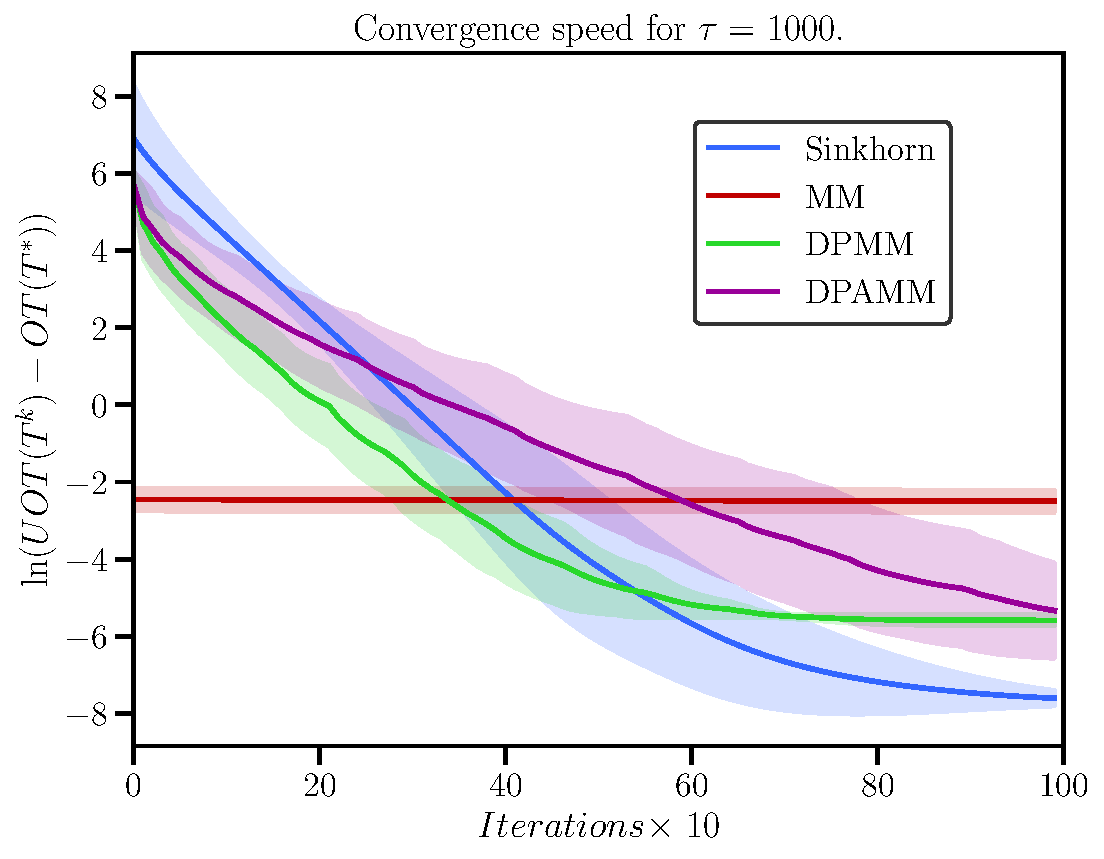
\includegraphics[width = 0.99\linewidth]{pic/ex1}
\centering
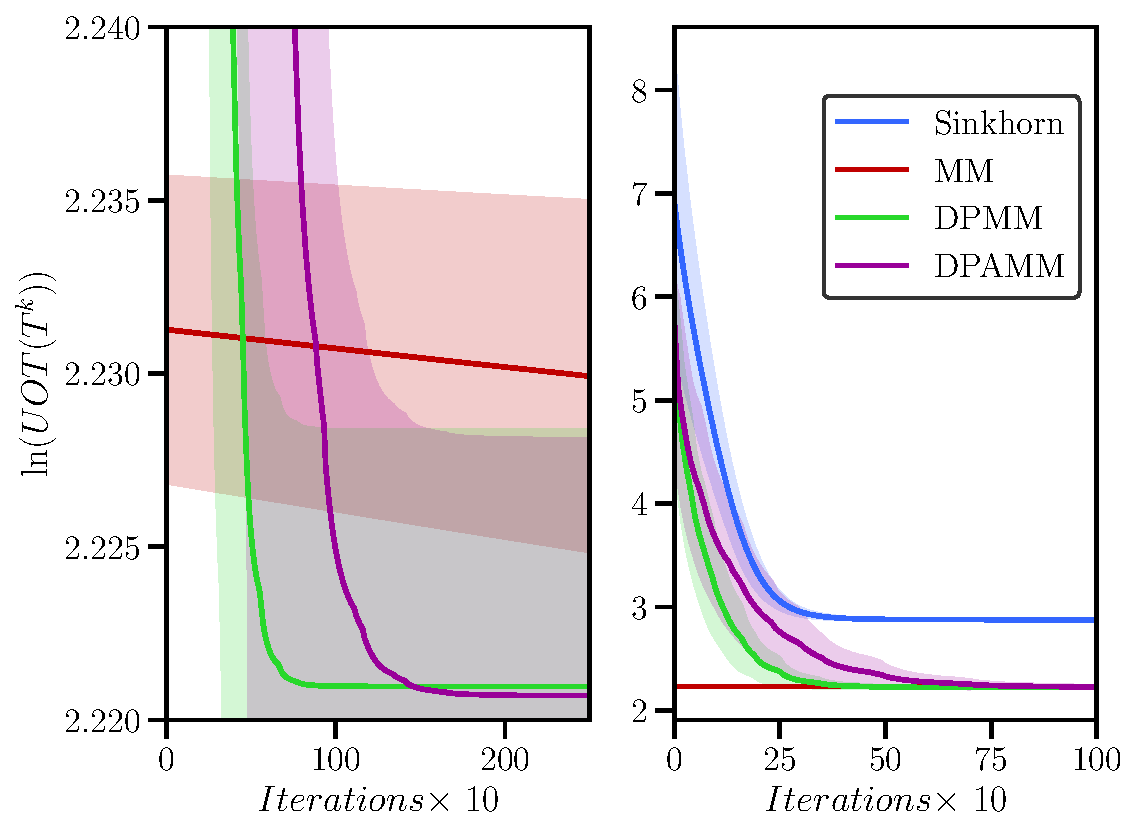
\includegraphics[width = 0.99\linewidth]{pic/ex3}
\caption{Comparison of the convergence speed for different algorithms. The upper plot represents the results for balanced samples, while the lower plot displays the results for unbalanced samples. Using $\operatorname{OT}(\mat T^{*})$ to represents the value of {(\ref{Eq:Standard_OT})}, and $\operatorname{UOT}(\mat T^{k})$ to represents the function value calculated by replacing the optimal $\mat T$ in {(\ref{eq:uot})} with $\mat T^{k}$ }
\label{Fig:ex1}
\end{figure}



\section{Experiments}

We conducted experiments using randomly generated Gaussian distributions. In particular, we generated five pairs of 100-dimensional Gaussian distributions, each with the same mass. To test the performance of our approach in the case of unequal mass i.e., {\it unbalanced} samples, we multiplied the mass of $\vec a$ by 1.2. For the mass-equal case i.e., balanced samples, we obtained the analytical optimal solution $\mat T^{*}$ using linear programming. For both cases, we set $\tau = 1000$, and we set the regularizer parameter $\epsilon = 10^{-3}$ for Sinkhorn's algorithm. Additionally, we set the initial value of $\tilde{\tau} = 0.1$ and $q = 10^{-4}$ for our DPMM algorithm. We also incorporated the Nesterov acceleration into our DPMM algorithm to obtain an accelerated variant, which is called DPAMM. Fig.~\ref{Fig:ex1} presents the results of our experiments.


\begin{figure}[tp]
\centering
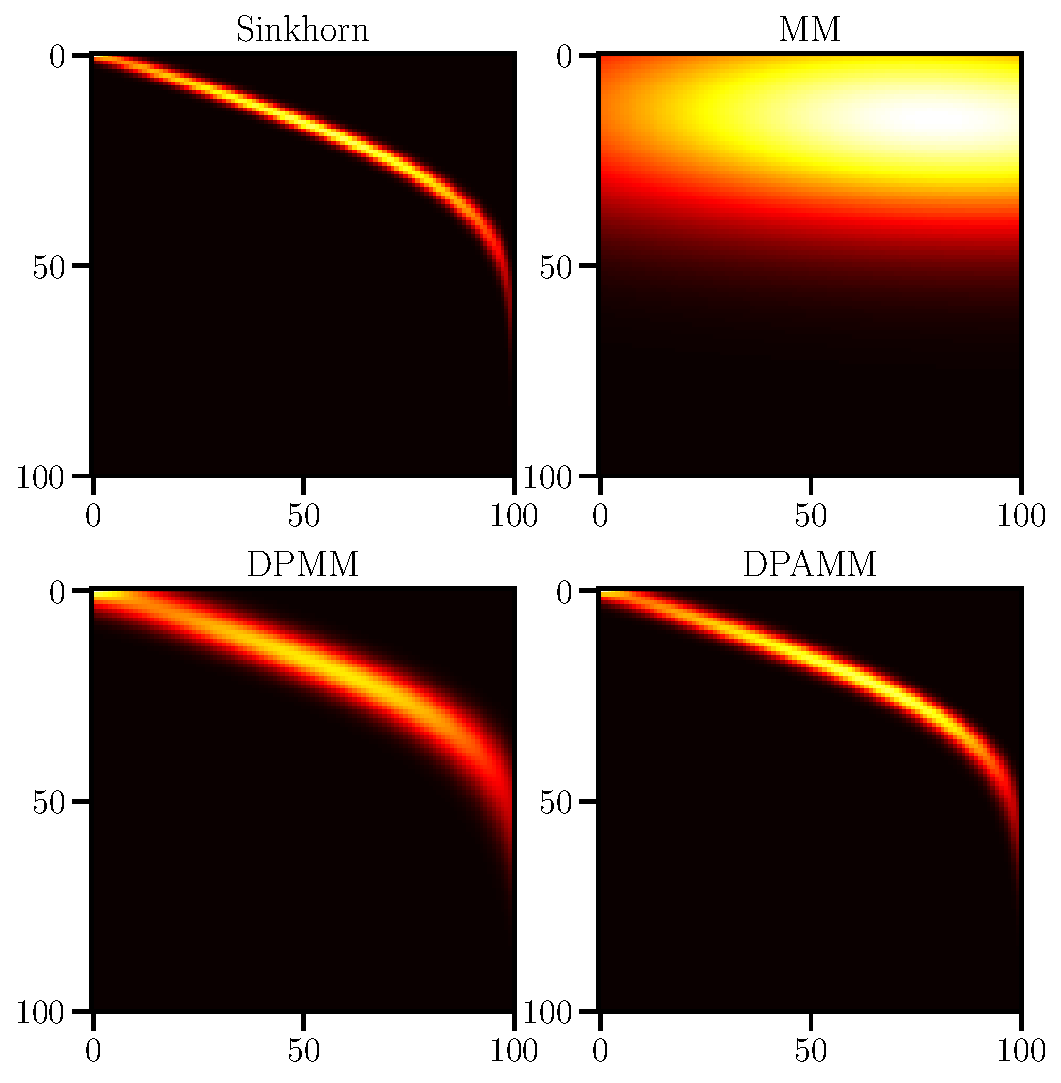
\includegraphics[width = 1.05\linewidth]{pic/ex2}
\centering
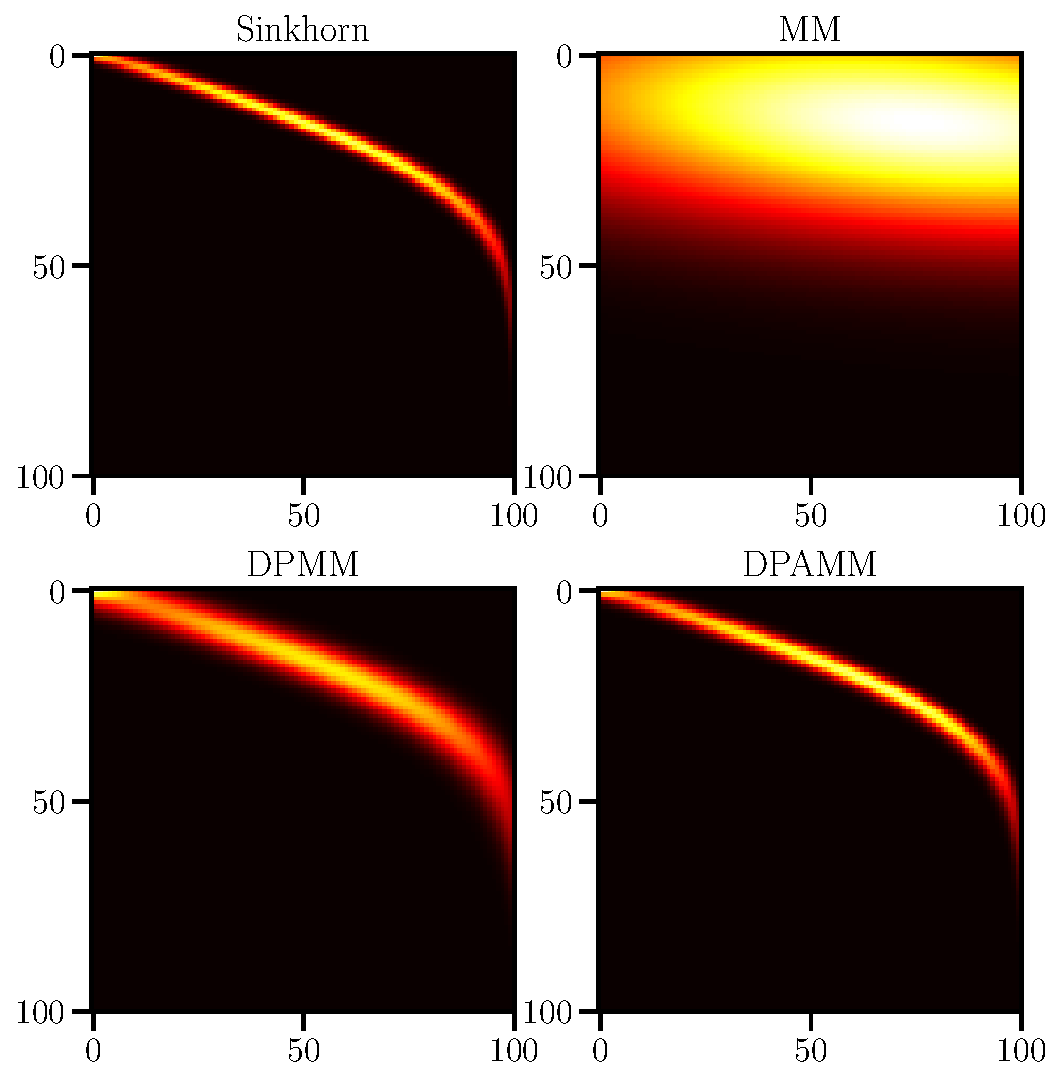
\includegraphics[width = 1.05\linewidth]{pic/ex4}
\setlength{\belowcaptionskip}{-30pt}
\caption{Comparison of the solutions obtained using different optimization methods over 1000 iterations, The upper plot represents the results for balanced samples, while the lower plot displays the results for unbalanced samples. The conventional MM algorithm fails to converge quickly to a near-sparse solution in any condition. Our proposed MM-IP and AMM-IP methods perform significantly better, producing solutions not only that have a similar structure to Sinkhorn's but also better accuracy for unbalanced samples.}
\label{Fig:ex2}
\end{figure}

The results indicate that the MM algorithm struggles to minimize the transport cost when dealing with a large penalization parameter, leading to significantly higher errors compared to other methods in balanced samples. In the case of unbalanced samples, the algorithm's convergence is extremely slow. As illustrated in Fig.~\ref{Fig:ex2}, the large value of $\tau$ causes the MM algorithm to preserve a blurry solution, which is inferior to both Sinkhorn's algorithm and our proposed methods. Our approach not only rapidly solves the problem with a clear structure similar to Sinkhorn's algorithm, but also maintains a small error for unbalanced samples, where Sinkhorn suffers from errors due to the regularizer.



\section{Conclusion}
\changeSX{We have centered our attention on the latest advancements in the optimization of UOT problems and used the BPD algorithm as an example to illustrate the MM algorithm's application. Our experimental results demonstrate the efficacy of our proposed DPMM algorithm.} Compared to the MM algorithm, our method effectively addresses the difficulties posed by larger values of $\tau$ by utilizing a dynamic penalization process that prevents poor initialization. As a result, we achieve a higher quality solution that competes with the well-known Sinkhorn's algorithm. In the future, we plan to leverage our expertise in the ALM domain to further enhance the performance of the MM algorithm.



\clearpage
\bibliographystyle{IEEEtran}
\bibliography{ref_new}
\color{red}

\end{document}
